        \documentclass{standalone}
        \usepackage{tikz}
        \usetikzlibrary{arrows}
        \usepackage{amsmath}
        \usepackage{amsfonts}
        \begin{document}
        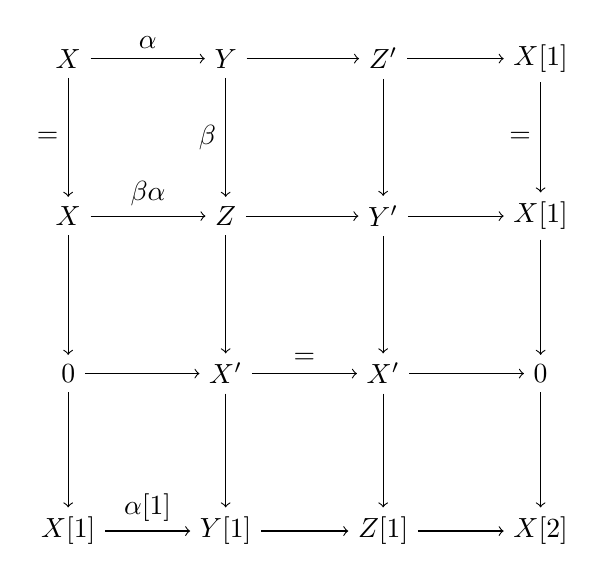
\begin{tikzpicture}

    \node (Xa) at (-4,2) {$X$};
    \node (Y) at (-2,2) {$Y$};
    \node (Z') at (0,2) {$Z^\prime$};
    \node (X1a) at (2,2) {$X[1]$};
    \node (Xb) at (-4,0) {$X$};
    \node (Z) at (-2,0) {$Z$};
    \node (Y') at (0,0) {$Y^\prime$};
    \node (X1b) at (2,0) {$X[1]$};
    \node (02) at (-4,-2) {$0$};
    \node (X'a) at (-2,-2) {$X^\prime$};
    \node (X'b) at (0,-2) {$X^\prime$};
    \node (03) at (2,-2) {$0$};
    \node (X1) at (-4,-4) {$X[1]$};
    \node (Y1) at (-2,-4) {$Y[1]$};
    \node (Z1) at (0,-4) {$Z[1]$};
    \node (X2) at (2,-4) {$X[2]$};
    \draw[->] (Xa) -- node[above] {$\alpha$} (Y);
    \draw[->] (Y) -- (Z');
    \draw[->] (Z') -- (X1a);
    \draw[->] (Xa) -- node[left] {$=$} (Xb);
    \draw[->] (Y) -- node[left] {$\beta$} (Z); 
    \draw[->] (Z') -- (Y');
    \draw[->] (X1a) -- node[left] {$=$} (X1b);\
    \draw[->] (Xb) -- node[above] {$\beta \alpha$} (Z);
    \draw[->] (Z) -- (Y');
    \draw[->] (Y') -- (X1b);
    \draw[->] (Xb) -- (02);
    \draw[->] (Z) -- (X'a);
    \draw[->] (Y') -- (X'b);
    \draw[->] (X1b) -- (03);
    \draw[->] (02) -- (X'a);
    \draw[->] (X'a) -- node[above] {$=$} (X'b); 
    \draw[->] (X'b) -- (03);
    \draw[->] (02) -- (X1);
    \draw[->] (X'a) -- (Y1);
    \draw[->] (X'b) -- (Z1);
    \draw[->] (03) -- (X2);
    \draw[->] (X1) -- node[above] {$\alpha[1]$} (Y1);
    \draw[->] (Y1) -- (Z1);
    \draw[->] (Z1) -- (X2); 
        \end{tikzpicture}
        \end{document}
